\section{Auswertung und Diskussion}
\label{sec:Auswertung}

In den nachfolgenden Abbildungen ist die sich ergebene Dosisverteilung aus verschiedenen
Ansichten dargestellt. In Abbildung \ref{abb:Z} die Transversalansicht, in Abbildung \ref{abb:Y} die
Frontalansicht und in Abbildung \ref{abb:X} die Sagittalansicht.


\begin{figure}[H]
  \centering
  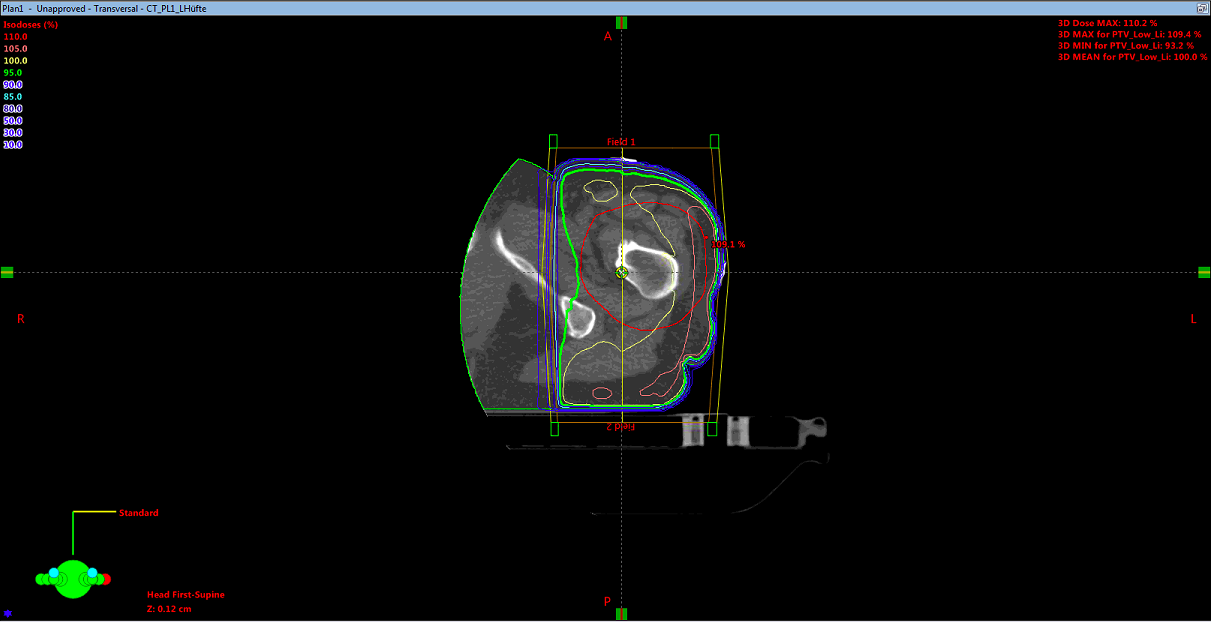
\includegraphics[width=\textwidth]{Bilder/HüfteZ.png}
  \caption{Darstellung der Dosisverteilung im Fuß in Transversalansicht.}
  \label{abb:Z}
\end{figure}

\begin{figure}[H]
  \centering
  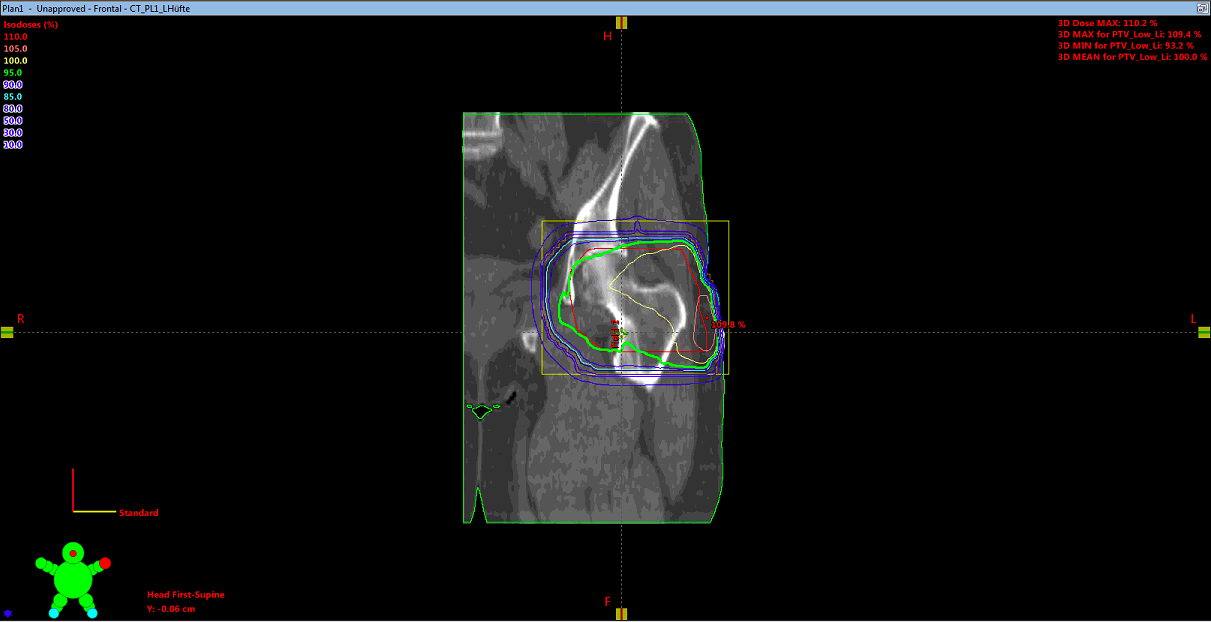
\includegraphics[width=\textwidth]{Bilder/HüfteY.png}
  \caption{Darstellung der Dosisverteilung im Fuß in Frontalansicht.}
  \label{abb:Y}
\end{figure}

\begin{figure}[H]
  \centering
  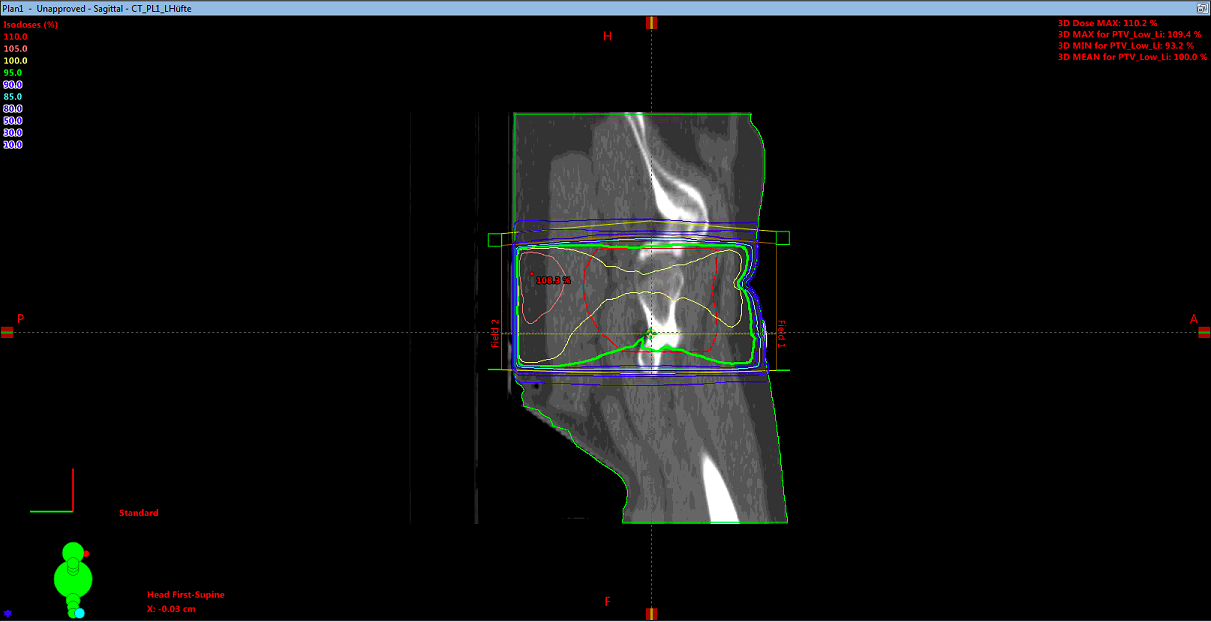
\includegraphics[width=\textwidth]{Bilder/HüfteX.png}
  \caption{Darstellung der Dosisverteilung im Fuß in Sagittalansicht.}
  \label{abb:X}
\end{figure}

Anhand der verschiedenen Ansichten von der Dosisverteilung ist zu erkennen, dass das
PTV weitgehend von der $95\%$ Isodosenlinie umschlossen ist. An den Stellen, wo die $95\%$ Isodosenlinie innerhalb
des PTVs verläuft werden die Strahlenfelder durch den Oberschenkelknochen abgeschwächt. Allerdings ist dies nur an
wenigen Stellen der Fall. Es fällt allerdings auf, dass außerhalb des PTVs eine hohe relative Dosis von über $100\%$ deponiert wird.
Außerdem liegt die maximale relative Dosis $110,2\%$ in dem gesunden Gewebe. Diese maximale Dosis
ist um $3,2\%$ größer als die erlaubte maximale Dosis von $107\%$ \cite{ICRU}. Bei dieser Therapie mit relativ geringen Fraktionsdosen
bestrahlt und deshalb wird es durch diese hohe relative Dosis zu keiner Schädigung des gesunden Gewebes kommen. Des weiteren
liegen im unmittelbaren Umfeld keine Risikoorgane, die geschädigt werden könnten.
Die maximale Dosis, die im PTV deponiert wird beträgt $109,7\%$. Diese liegt auch oberhalb der erlaubten maximalen Dosis, aber
wie bereits erwähnt kann diese maximale Dosis aufgrund der geringen Fraktionsdosen toleriert werden.
In dem PTV wird mindestens eine relative Dosis von $93,2\%$ deponiert. Diese liegt etwas unterhalb der gewünschten $95\%$ und
wird vermutlich an den Stellen des PTV deponiert, die in Knochen liegen.
Zur genaueren Beurteilung der Dosisverteilung ist in Abbildung \ref{abb:DVH} das DVH für das
PTV (rot) und den Körper (grün) dargestellt.


\begin{figure}[H]
  \centering
  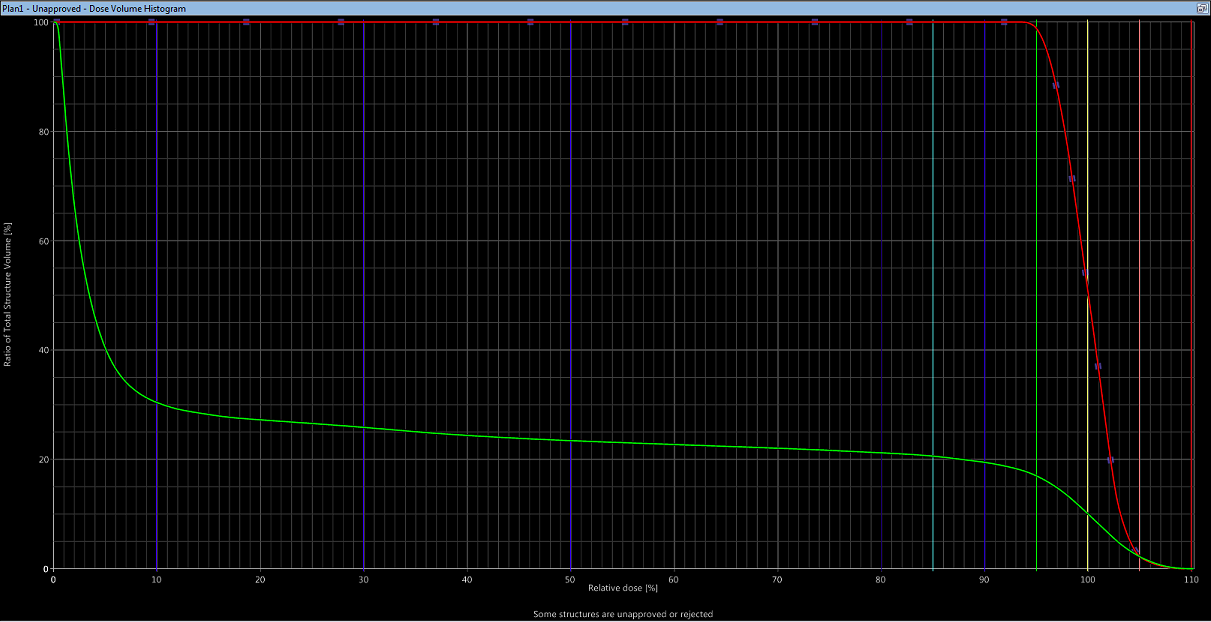
\includegraphics[width=\textwidth]{Bilder/DVH_HüfteEinzel.png}
  \caption{Dosis-Volumen-Histogramm für das PTV in rot und den gesamten Körper, der in dem CT-Bild abgebildet ist, in grün.}
  \label{abb:DVH}
\end{figure}

Anhand des DVHs von dem PTV ist zu erkennen, dass in etwa $98\%$ des PTVs $95\%$ der relativen Dosis deponiert wird. Es
ist auch zu erkennen, dass nur ein sehr geringer Teil des PTVs eine Dosis von über $107\%$ erhält.
Das DVH des gesamten Körpervolumens zeigt, dass etwa $27\%$ des Volumens eine relative Dosis von $20\%$ erhält und noch etwa $24\%$ des Volumens
eine Dosis von $50\%$. Das konnte auch schon anhand der Dosisverteilung gesehen werden, dass auch im gesunden Gewebe eine relativ hohe Dosis deponiert wird.
Allerdings ist auch zu erkennen, dass weniger als $10\%$ des gesamten Volumens eine Dosis von über $100\%$ erhält. \\

Mit der gewählten Feldkonfiguration konnte das Ziel, das PTV mit der $95\%$ Isodosenlinie zu umschließen, gut erreicht werden.
Durch die verwendeten MLCs konnte das gesunde Gewebe etwas geschützt werden, allerdings wird dort trotzdem eine
relativ hohe Dosis deponiert. Da es sich bei dieser Therapie allerdings nur geringe Fraktionsdosen handelt,
kann diese hohe Dosisdeposition im gesunden Gewebe toleriert werden. 
